\documentclass[nooutcomes]{ximera}
%% handout
%% space
%% newpage
%% numbers
%% nooutcomes

%I added the commands here so that I would't have to keep looking them up
%\newcommand{\RR}{\mathbb R}
%\renewcommand{\d}{\,d}
%\newcommand{\dd}[2][]{\frac{d #1}{d #2}}
%\renewcommand{\l}{\ell}
%\newcommand{\ddx}{\frac{d}{dx}}
%\everymath{\displaystyle}
%\newcommand{\dfn}{\textbf}
%\newcommand{\eval}[1]{\bigg[ #1 \bigg]}

%\begin{image}
%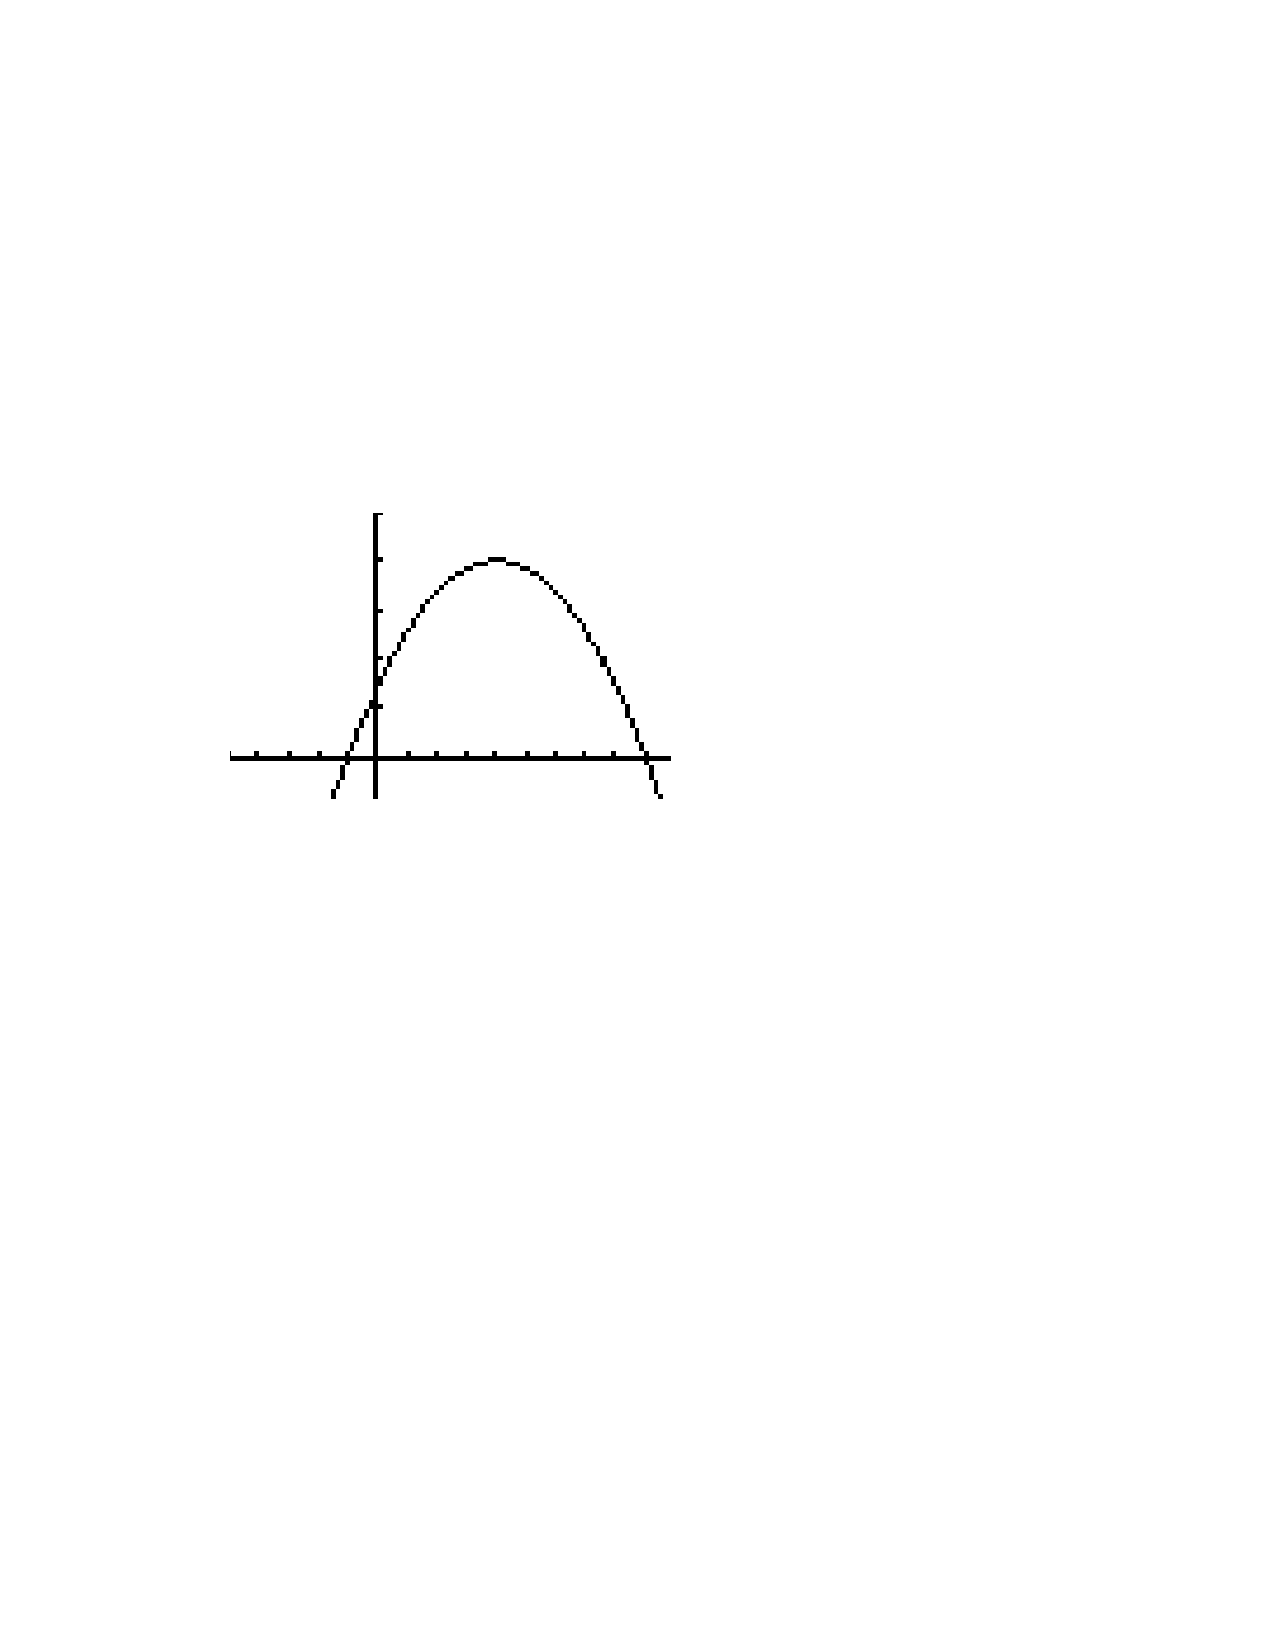
\includegraphics[trim= 170 420 250 180]{Figure1.pdf}
%\end{image}


\newcommand{\RR}{\mathbb R}
\renewcommand{\d}{\,d}
\newcommand{\dd}[2][]{\frac{d #1}{d #2}}
\renewcommand{\l}{\ell}
\newcommand{\ddx}{\frac{d}{dx}}
\newcommand{\dfn}{\textbf}
\newcommand{\eval}[1]{\bigg[ #1 \bigg]}

\usepackage{multicol}

\renewenvironment{freeResponse}{
\ifhandout\setbox0\vbox\bgroup\else
\begin{trivlist}\item[\hskip \labelsep\bfseries Solution:\hspace{2ex}]
\fi}
{\ifhandout\egroup\else
\end{trivlist}
\fi} %% we can turn off input when making a master document

\title{Recitation \#14 - 3.11 Related Rates (Solutions)}  

\begin{document}
\begin{abstract}		\end{abstract}
\maketitle

\section*{Warm up:} 
Find the mistake in the solution to the given problem:

Two boats leave from the same dock, but at slightly different times.  One boat is traveling east at 30mph while the other boat is traveling north at 15mph.  At an instant in time when the boat traveling east is 15 miles from the dock and the boat traveling north is 10 miles away from the dock, what rate is the distance between the boats changing?

	\begin{image}
	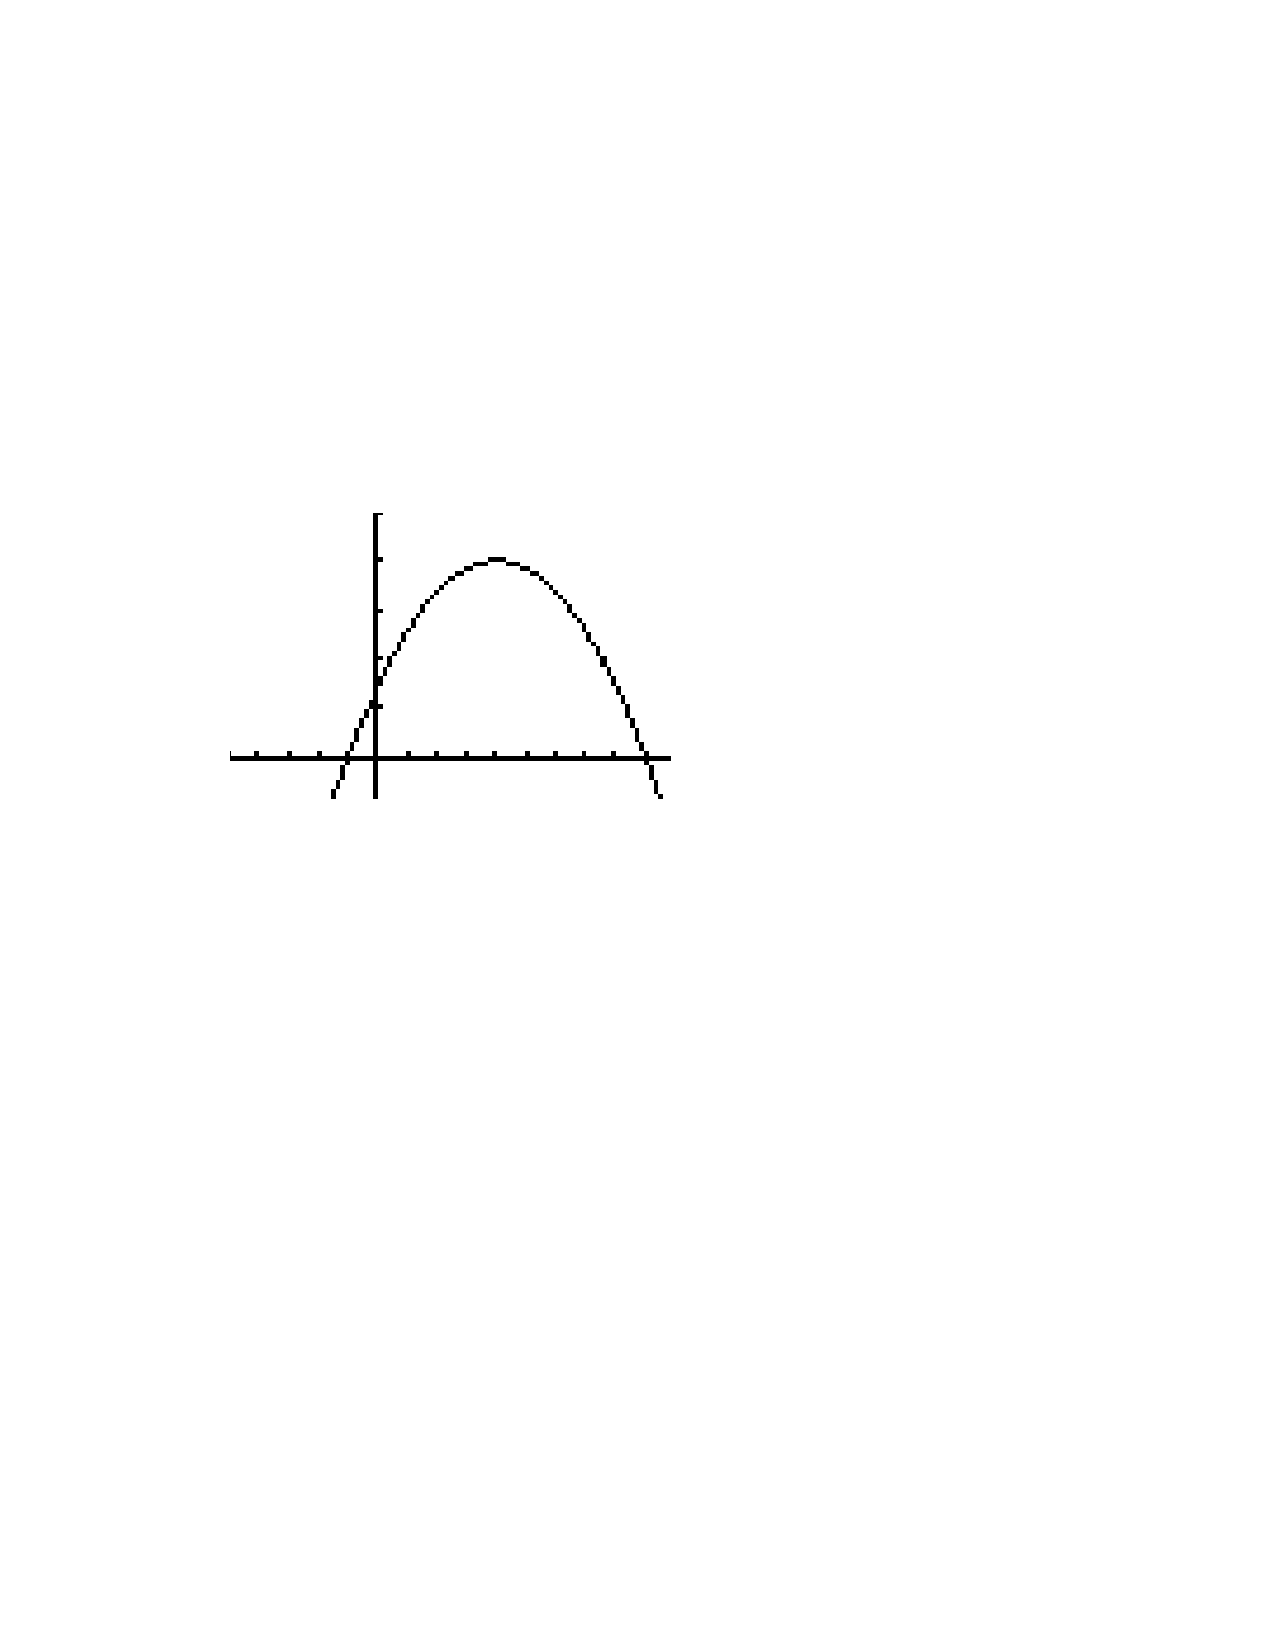
\includegraphics[trim= 170 350 250 90]{Figure1.pdf}
	\end{image}
	
		\begin{freeResponse}
		The error occurs when the student plugs in values for $x$ and $y$ \dfn{before} differentiating the equation $x^2 + y^2 = z^2$ with respect to time.  The distances $x$ and $y$ are clearly changing with respect to time, and so they cannot be treated as constants when we are differentiating.
		
		Differentiating $x^2 + y^2 = z^2$ with respect to $t$ yields:
		$$ 2x \dd[x]{t} + 2y \dd[y]{t} = 2z \dd[z]{t}$$
		
		Canceling the 2's and plugging in the known quantities yields:
		$$ z \dd[z]{t} = (15)(30) + (10)(15) = 450 + 150 = 600 $$
		
		In the above work, the student did correctly compute that $z^2 = 325$ at this fixed instant in time.  So $z = 5\sqrt{13}$, and we can solve for $\dd[z]{t}$ to obtain
		$$ \dd[z]{t} = \frac{600}{5 \sqrt{13}} = \frac{120}{\sqrt{13}} \, mph $$
		\end{freeResponse}	
		
		
		

	
	
	
	
	

\section*{Group work:}

	\begin{image}
	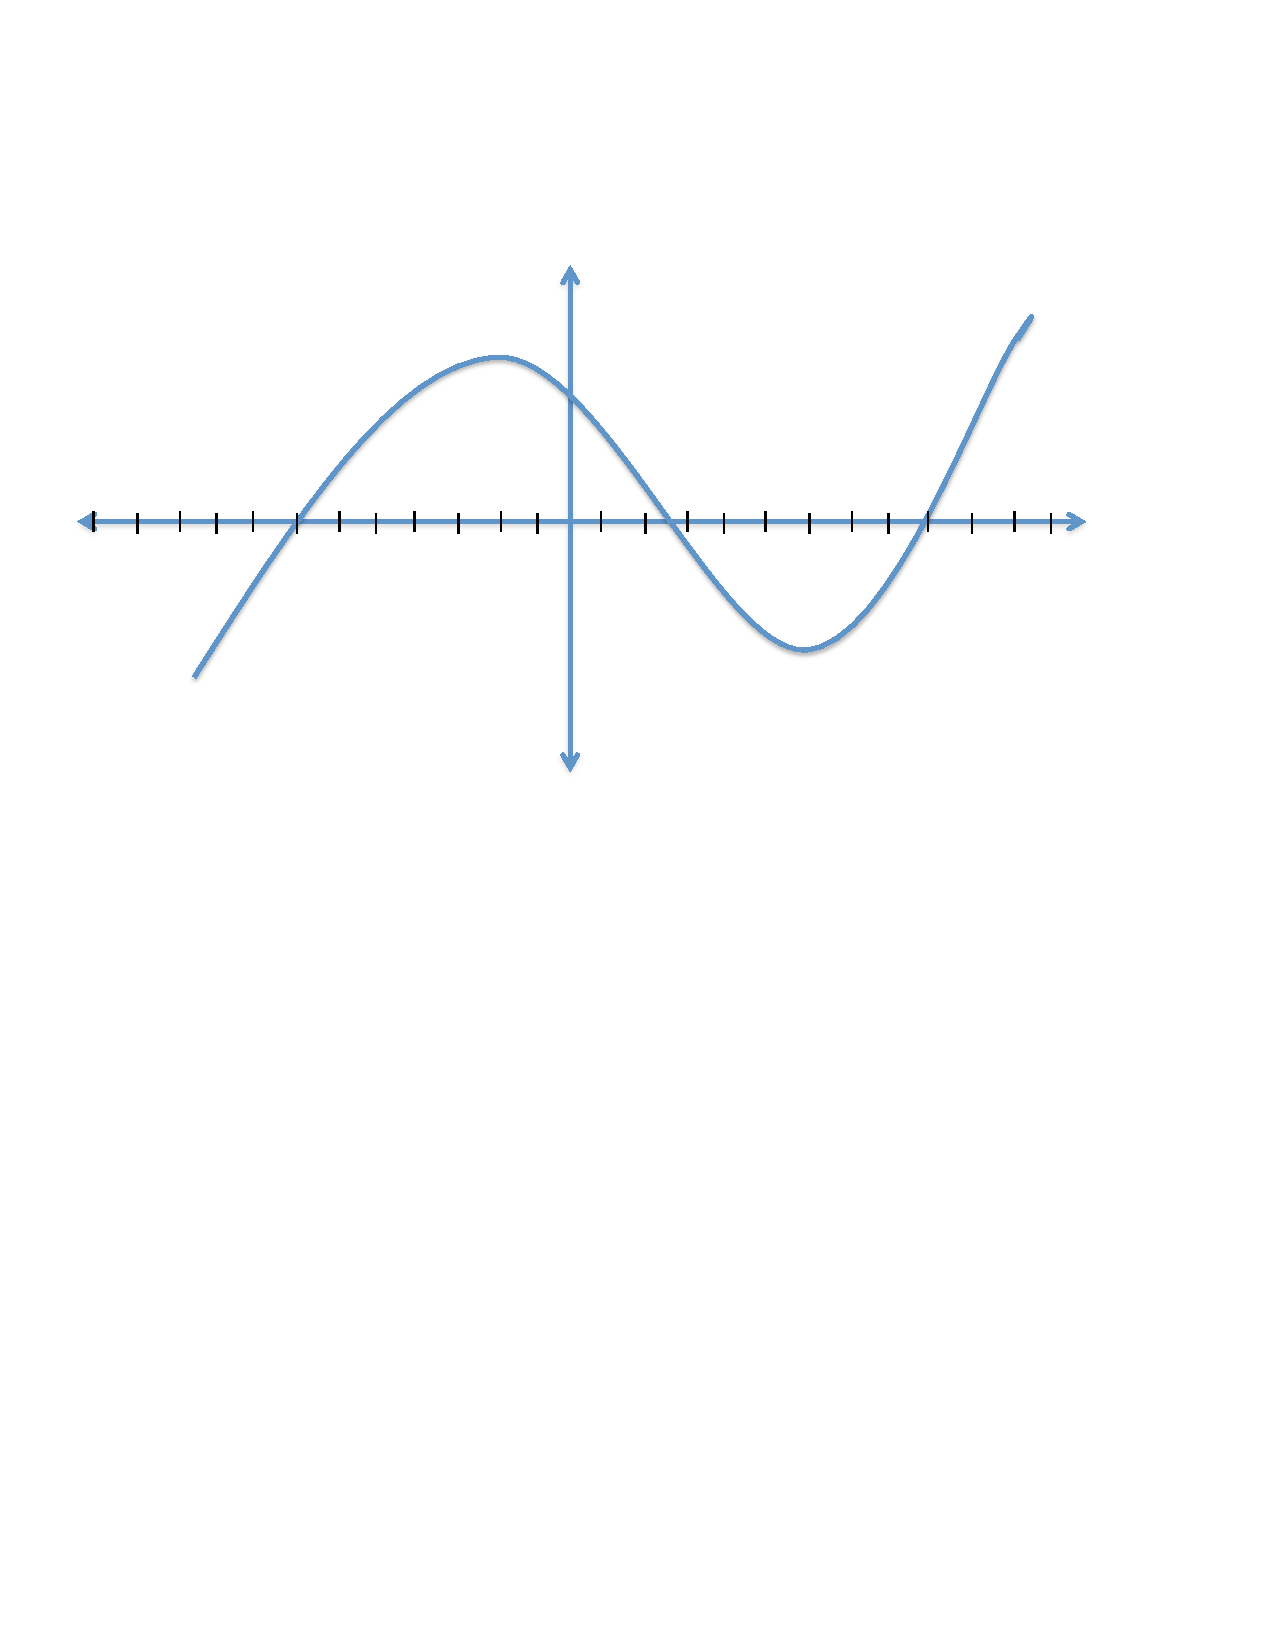
\includegraphics[trim= 220 480 250 90]{Figure2.pdf}
	\end{image}

%problem 1
\begin{problem}
An oil spill is being cleaned up by the deployment of bacteria that consume the oil at 3 cubic feet per hour.  The oil spill itself is modeled in the form of a very thin cylinder with height $h$ being the thickness of the oil slick (see the picture below).  Suppose at some moment in time, the height is decreasing at 0.0005 feet per hour, the thickness of the slick is 0.007 feet, and the cylinder is 900 feet in diameter.  At what rate is the area covered by the slick changing at that moment (that is, the area of the base disc of the cylinder)?
	\begin{image}
	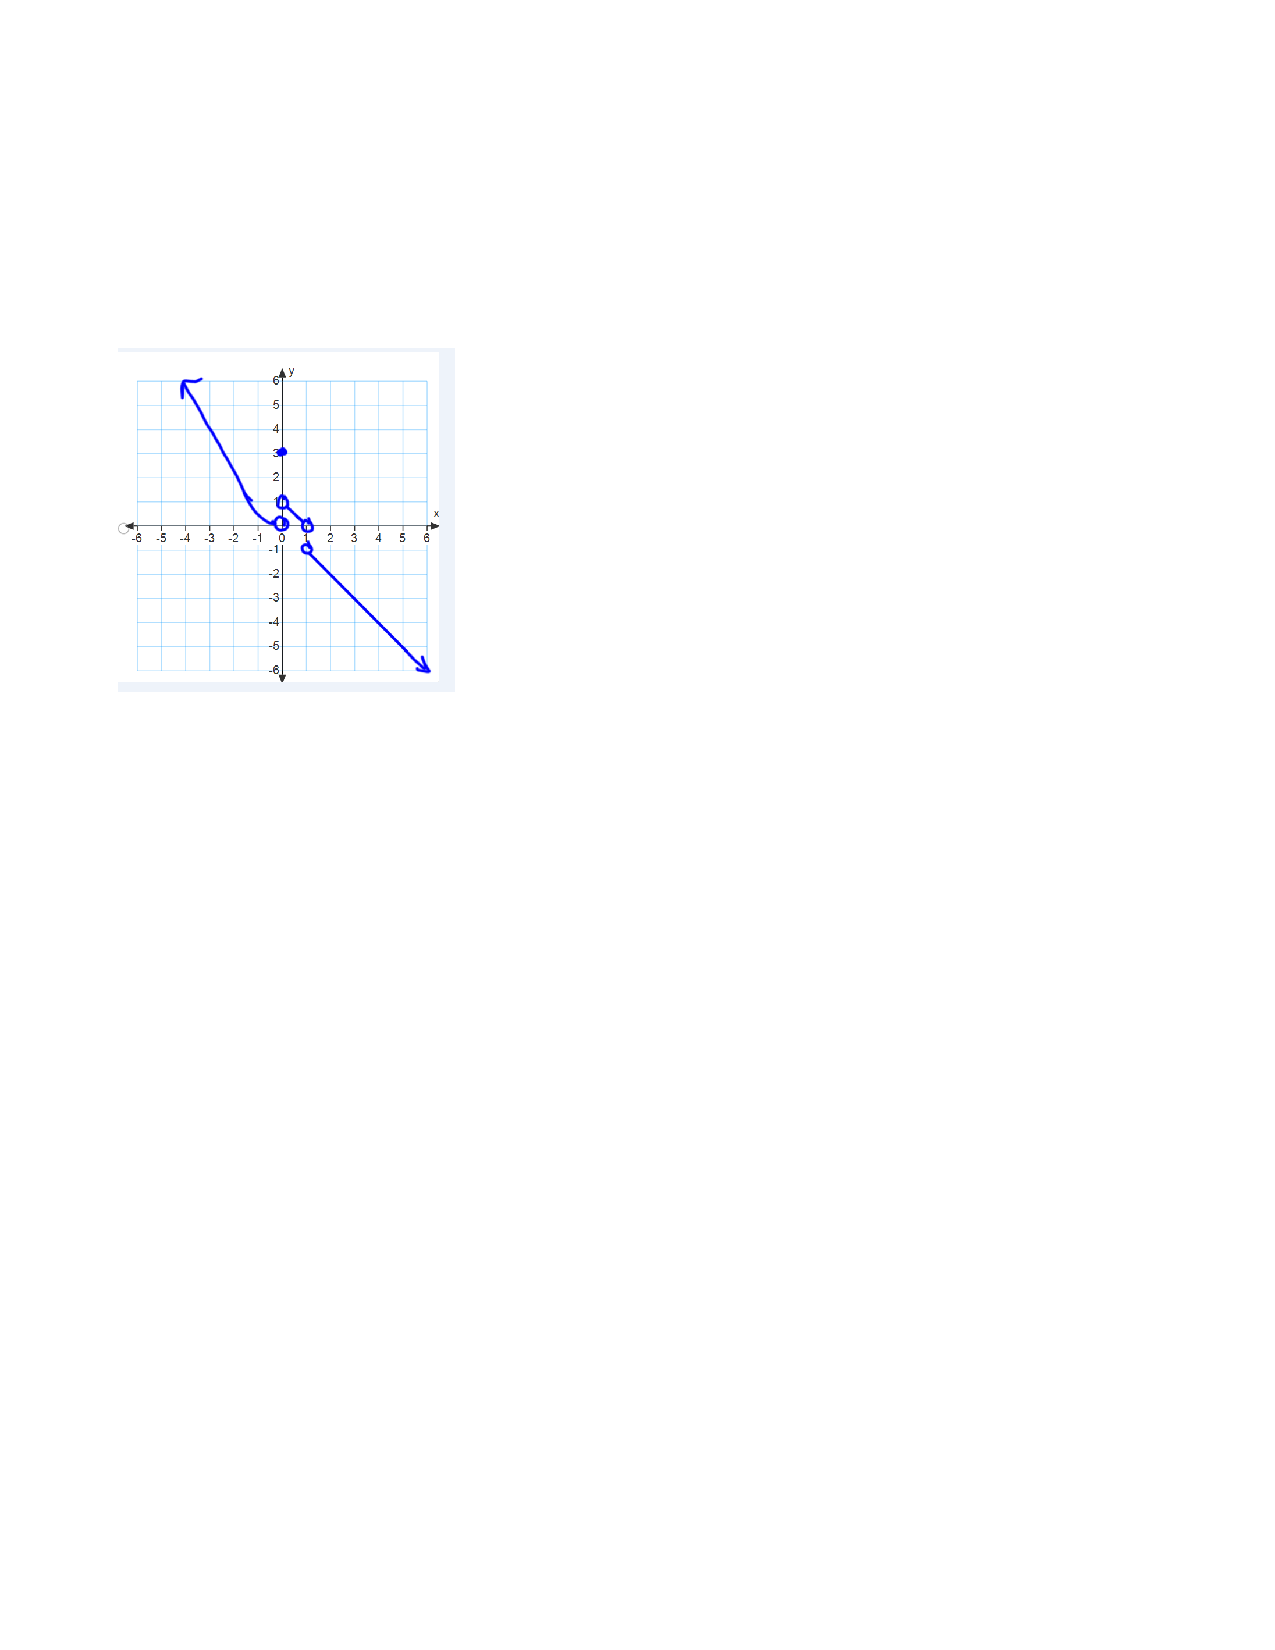
\includegraphics[trim= 100 520 250 220]{Figure3.pdf}
	\end{image}
	
		\begin{freeResponse}
		Let $V$ denote the volume, $A$ denote the area of the base, $h$ denote the height (or thickness), and $r$ denote the radius of the oil slick.  Note that the first piece of information that we are given is that $\dd[V]{t} = -3 \, \frac{ft^3}{hr}$.  
		
		Let $t_0$ denote the instant in time that we are concerned about.  Then at time $t_0$ we are also given that:
		$$ \dd[h]{t} = \left( -5 \times 10^{-4} \right) \frac{ft}{hr}  \qquad  h = \left( 7 \times 10^{-3} \right) ft  \qquad  r = \left( 4.5 \times 10^2 \right) ft $$
		and the problem asks us to find $\dd[A]{t}$ at time $t_0$.  
		
		Since $A = \pi r^2$, we have that $\dd[A]{t} = 2 \pi r \dd[r]{t}$.  So at time $t_0$ we have that $\dd[A]{t} = 900 \pi \dd[r]{t}$.  Unfortunately, we are not given $\dd[r]{t}$ at time $t_0$, and so our goal now is to find this.
		
		Since $V = \pi r^2 h$, we can use the product rule to compute
		\begin{equation}\label{dVdtprob1}
		\dd[V]{t} = \pi \left( 2r \dd[r]{t} h + r^2 \dd[h]{t} \right)
		\end{equation}
		
		Using all of our known quantities, we can plug into equation \ref{dVdtprob1} and solve for $\dd[r]{t}$ at time $t_0$:
		$$ -3 = \pi \left( 2(450)(7 \times 10^{-3}) \dd[r]{t} + (4.5 \times 10^2)^2(-5 \times 10^{-4}) \right) $$
		$$ -3 = \pi \left( 900(7 \times 10^{-3}) \dd[r]{t} + (20.25 \times 10^4) (-5 \times 10^{-4}) \right) $$
		$$ -3 = 6.3 \pi \dd[r]{t} -101.25 \pi $$
		$$ \dd[r]{t} = \frac{101.25 \pi - 3}{6.3 \pi} $$
		
		Thus, we solve
		$$ \dd[A]{t} = 900 \pi \cdot \frac{101.25 \pi - 3}{6.3 \pi} \, \frac{ft^2}{hr} = 900 \left( \frac{101.25 \pi - 3}{6.3} \right) \, \frac{ft^2}{hr} $$
		
		%another solution
		\dfn{Another Solution}
		
		Here is a very nice, but less obvious, solution to this problem.
		$V = \pi r^2 h = Ah$.  So 
		$$ \dd[V]{t} = \dd[A]{t} h + A \dd[h]{t} = \dd[A]{t} h + \pi r^2 \dd[h]{t}$$
		and thus
		$$ -3 = (7 \times 10^{-3}) \dd[A]{t} + \pi \cdot 450^2 \cdot (-5 \times 10^{-4}) $$
		$$ -3 = (7 \times 10^{-3}) \dd[A]{t} - 101.25 \pi  $$
		$$ \dd[A]{t} = \frac{101.25 \pi - 3}{7 \times 10^{-3}} \, \frac{ft^2}{hr} $$
		
		\end{freeResponse}
		
		
\end{problem}









%problem 2
\begin{problem}
A hot air balloon is 150 ft above the ground when a motorcycle passes directly beneath it traveling at a rate of 60 ft/sec (in a straight line on a horizontal road).  If the balloon is rising vertically at a rate of 10 ft/s, what is the rate of change of the distance between the motorcycle and the balloon 10 seconds later?
		\begin{freeResponse}
		Let $P$ denote the point on the ground directly below the hot air balloon, let $x$ denote the distance from the motorcycle to $P$, let $y$ denote the distance from the hot air balloon to $P$, and let $z$ denote the distance from the motorcycle to the hot air balloon.  The location of the motorcycle, the hot air balloon, and the point $P$ form a right triangle, and so we have that 
		\begin{equation}\label{Pythagorean}
		x^2 + y^2 = z^2.
		\end{equation}
		  We are given that $\dd[x]{t} = 60$ and $\dd[y]{t} = 10$, and the question asks us to find $\dd[z]{t}$ at time $t=10$ (meaning 10 seconds after the motorcycle passes the point $P$).  We can also easily compute that:
		$$ x(10) = 60 \cdot 10 = 600 ft $$
		$$ y(10) = 150 + (10 \cdot 10) = 250 ft $$
		$$ z(10) = \sqrt{ 600^2 + 250^2} = \sqrt{360000 + 62500} = \sqrt{422500} = 650 ft $$
		where $x(10), y(10), and $z(10) denote the values of $x$, $y$, and $z$ 10 seconds after the motorcycle passes the point $P$.  
		
		Differentiating equation \ref{Pythagorean} with respect to time, substituting, and solving for $\dd[z]{t}$ yields:
		$$ 2x \dd[x]{t} + 2y \dd[y]{t} = 2z \dd[z]{t} $$
		$$ x \dd[x]{t} + y \dd[y]{t} = z \dd[z]{t} $$
		$$ (600)(60) + (250)(10) = (650) \dd[z]{t} $$
		$$ \dd[z]{t} = \frac{36000 + 2500}{650} \frac{ft}{sec} = \frac{3850}{65} \frac{ft}{sec} = \frac{770}{13} \frac{ft}{sec} \approx 59.23 \frac{ft}{sec} $$
		
		\end{freeResponse}
			
			
		
\end{problem}















%problem 3
\begin{problem}
A swimming pool is 20 feet long and has transverse cross sections which look like the figure below.   If the pool is being filled at a rate of 0.8 cubic feet per minute, how fast is the water level rising when the depth of the water is 3 feet? 
	\begin{image}
	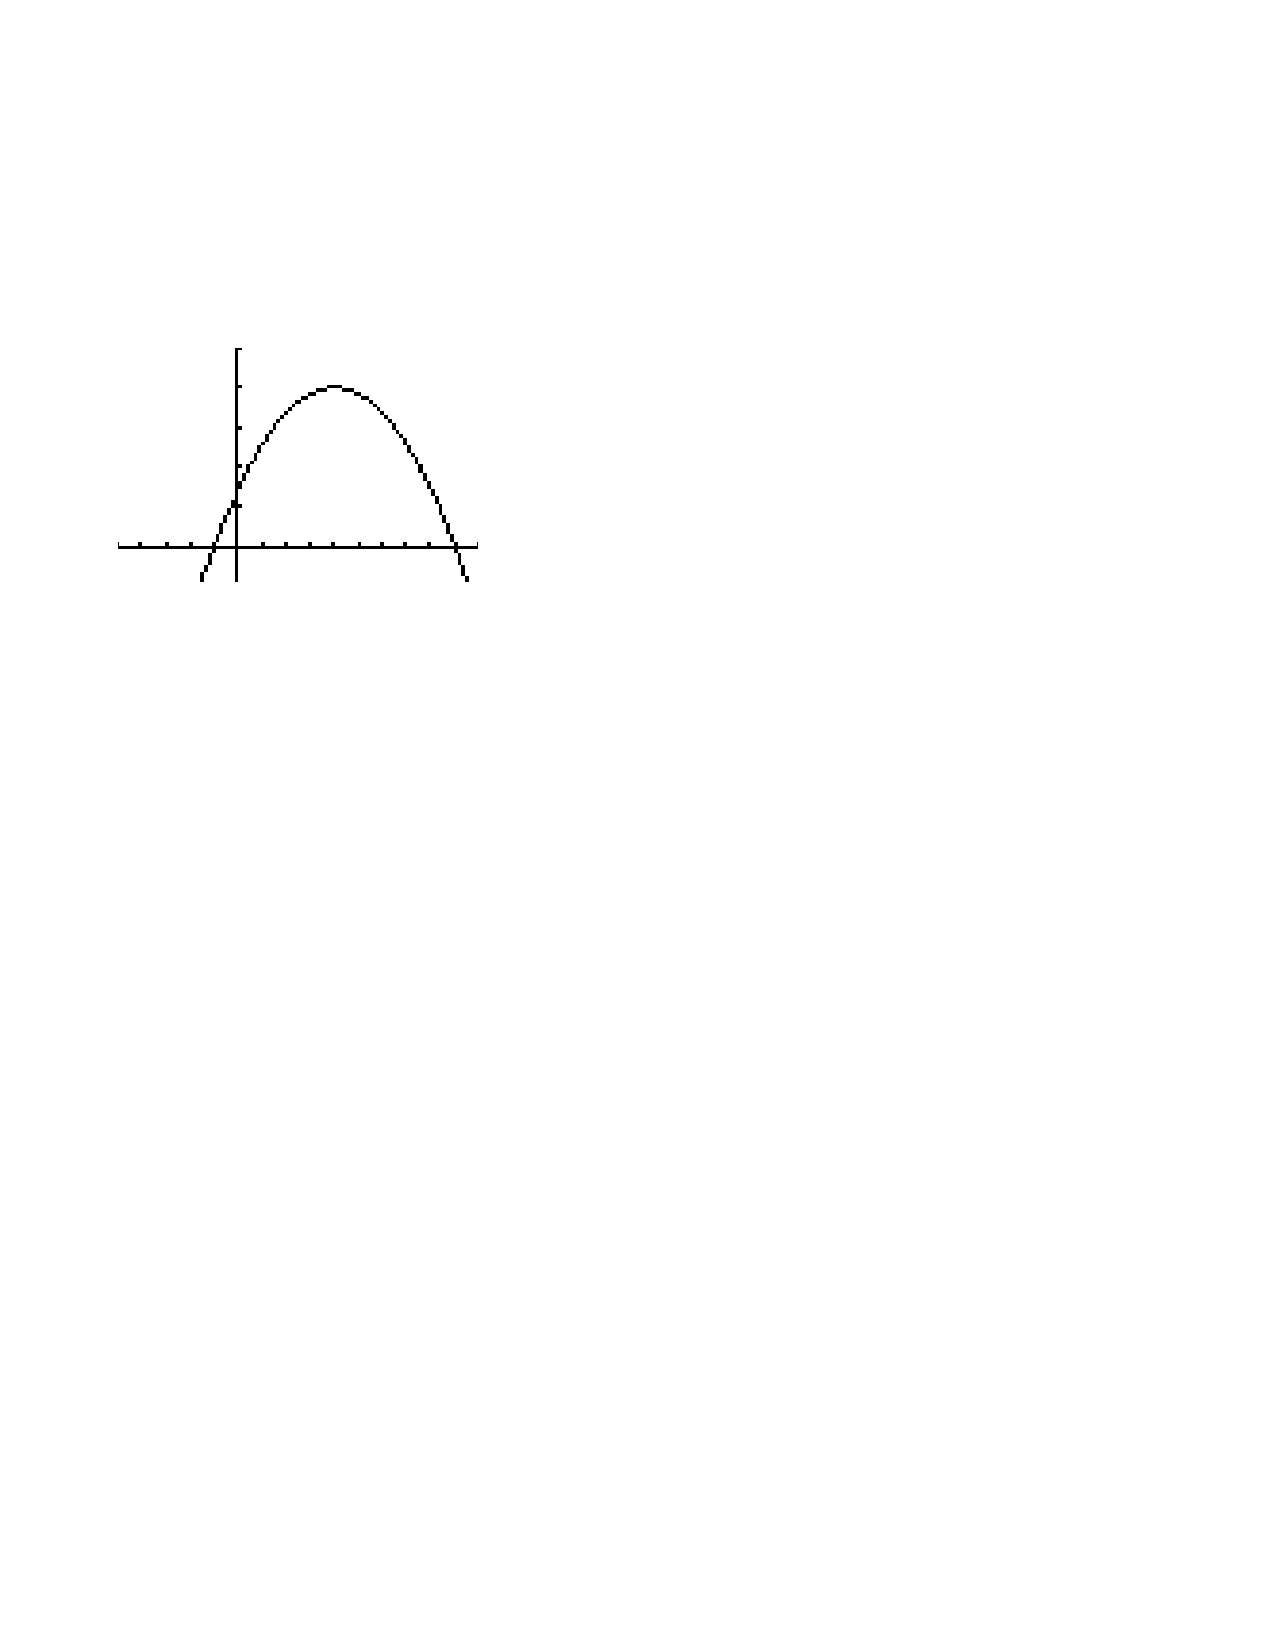
\includegraphics[trim= 100 500 250 170]{Figure4.pdf}
	\end{image}
	
		\begin{freeResponse}
		Let $V$ denote the volume and $h$ denote the height of the water in the pool.  We are given that the pool is being filled at a rate of $0.8$ cubic feet per minute, and so $\dd[V]{t} = \frac{4}{5} \frac{ft^3}{min}$.  We want to find $\dd[h]{t}$ at the instant in time when $h=3 ft$.  Since the height that we care about is below the height $h=6 ft$ where the pool changes shape, we only need to worry about the shape of the bottom of the pool.  This portion of the pool looks like:
		
		\begin{image}
		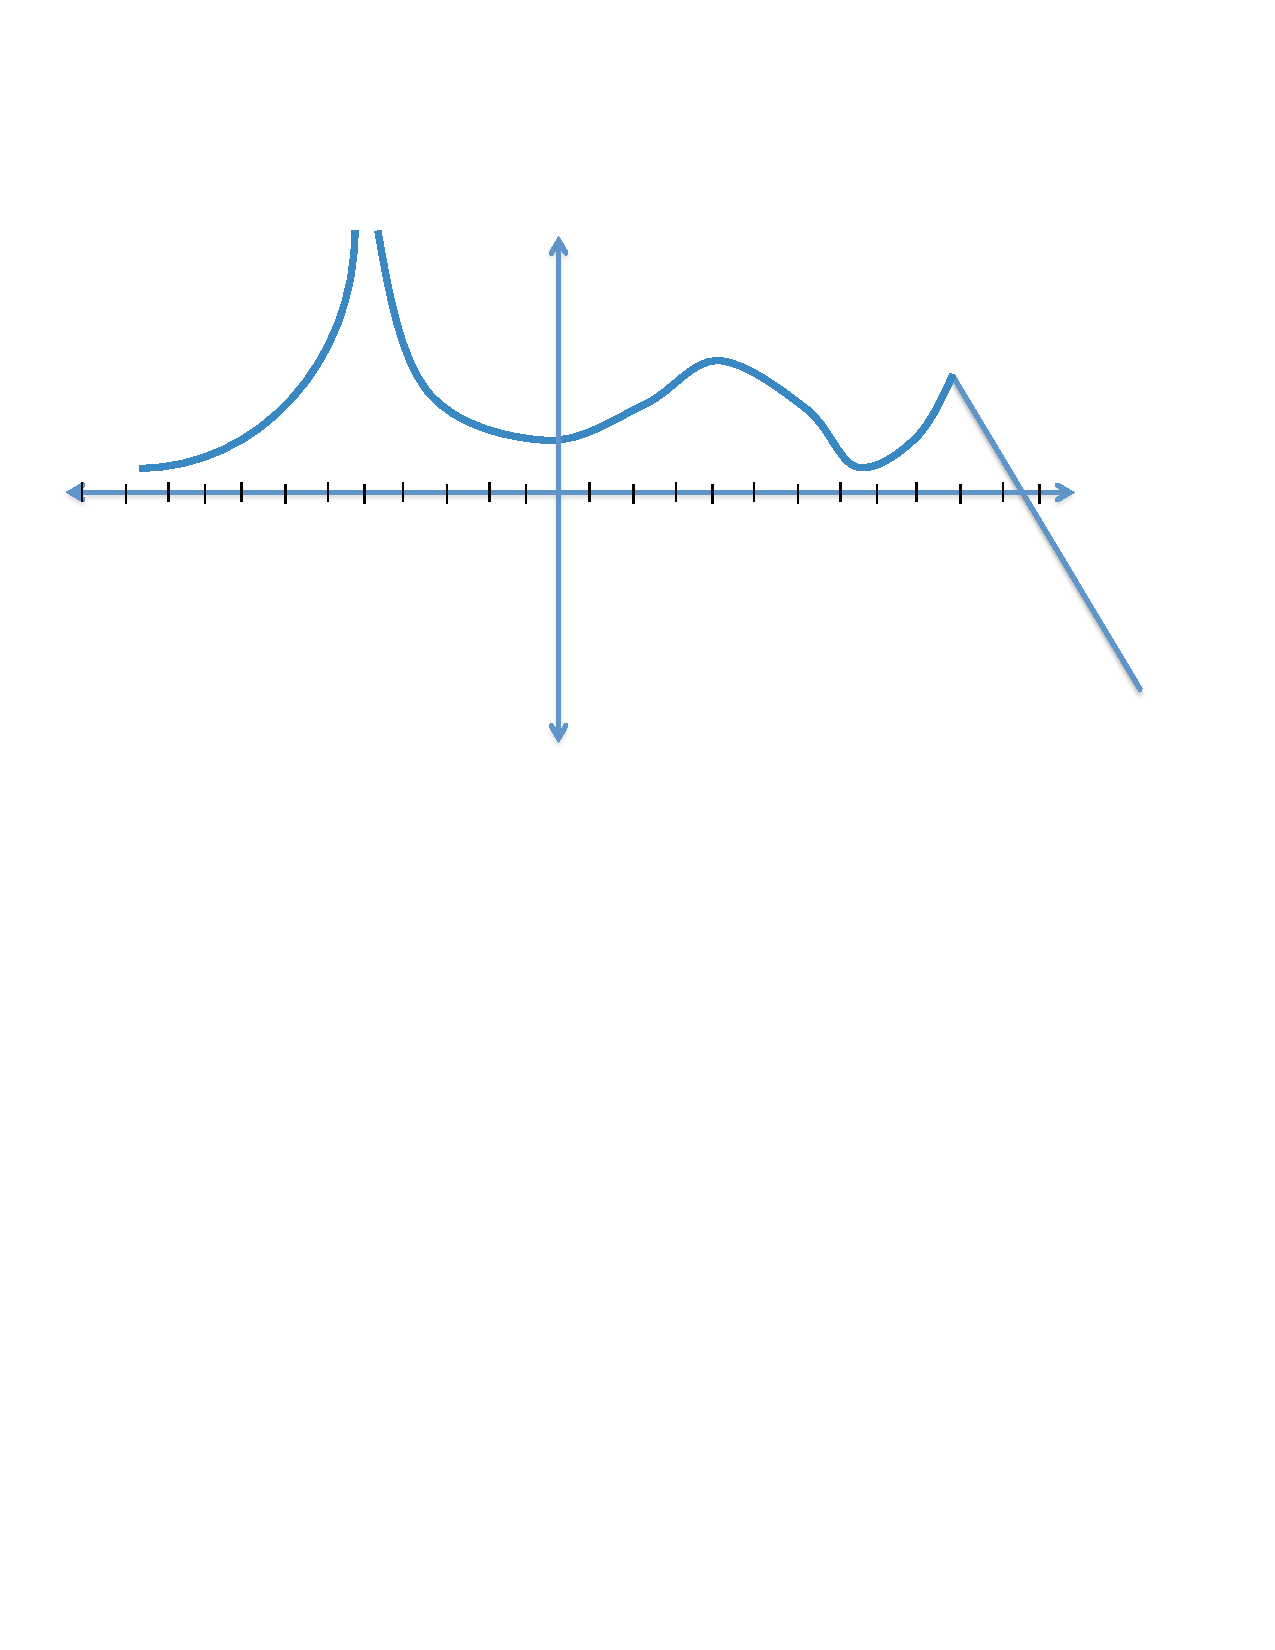
\includegraphics[trim= 100 500 250 200]{Figure5.pdf}
		\end{image}
		
		Observe that the volume of the water in the pool is
		\begin{equation}\label{Vprob2}
		V = 20 \left( 14h + 2 \left( \frac{1}{2} xh \right) \right) = 20 \left( 14h + xh \right)
		\end{equation}
		where $x$ is as in the picture above, and the 20 is due to the length of the pool.  
		
		We could attempt to solve for $\dd[h]{t}$ by differentiating equation \ref{Vprob2} with respect to time, but the problem is that we do not know $\dd[x]{t}$.  So we need to use the geometry of the problem to write $x$ as a function of $h$.  And we do that here by using similar triangles.  Notice that $\frac{x}{h} = \frac{3}{6} = \frac{1}{2}$, and so $x = \frac{1}{2} h$.  Substituting this into equation \ref{Vprob2} yields:
		$$ V = 20 \left( 14h + \frac{1}{2} h^2 \right) $$
		
		Now we differentiate with respect to time, substitute, and solve for $\dd[h]{t}$:
		$$ \dd[V]{t} = 20 \left( 14 \dd[h]{t} + h \dd[h]{t} \right) $$
		$$ \frac{4}{5} = 20 \left( 14 \dd[h]{t} + 3 \dd[h]{t} \right) $$
		$$ \frac{4}{5} = 340 \dd[h]{t} $$
		$$ \dd[h]{t} = \frac{4}{5 \cdot 340} \frac{ft}{min} = \frac{1}{5 \cdot 85} \frac{ft}{min} = \frac{1}{425} \frac{ft}{min}. $$
		
		\end{freeResponse}
		
		
		

\end{problem}
	
	
	
	
	
	
	
	
			
			















	
	
	
	
	
	
	
	
	

	










								
				
				
	














\end{document} 


















